% This is "sig-alternate.tex" V2.0 May 2012
% This file should be compiled with V2.5 of "sig-alternate.cls" May 2012
%
% This example file demonstrates the use of the 'sig-alternate.cls'
% V2.5 LaTeX2e document class file. It is for those submitting
% articles to ACM Conference Proceedings WHO DO NOT WISH TO
% STRICTLY ADHERE TO THE SIGS (PUBS-BOARD-ENDORSED) STYLE.
% The 'sig-alternate.cls' file will produce a similar-looking,
% albeit, 'tighter' paper resulting in, invariably, fewer pages.
%
% ----------------------------------------------------------------------------------------------------------------
% This .tex file (and associated .cls V2.5) produces:
%       1) The Permission Statement
%       2) The Conference (location) Info information
%       3) The Copyright Line with ACM data
%       4) NO page numbers
%
% as against the acm_proc_article-sp.cls file which
% DOES NOT produce 1) thru' 3) above.
%
% Using 'sig-alternate.cls' you have control, however, from within
% the source .tex file, over both the CopyrightYear
% (defaulted to 200X) and the ACM Copyright Data
% (defaulted to X-XXXXX-XX-X/XX/XX).
% e.g.
% \CopyrightYear{2007} will cause 2007 to appear in the copyright line.
% \crdata{0-12345-67-8/90/12} will cause 0-12345-67-8/90/12 to appear in the copyright line.
%
% ---------------------------------------------------------------------------------------------------------------
% This .tex source is an example which *does* use
% the .bib file (from which the .bbl file % is produced).
% REMEMBER HOWEVER: After having produced the .bbl file,
% and prior to final submission, you *NEED* to 'insert'
% your .bbl file into your source .tex file so as to provide
% ONE 'self-contained' source file.
%
% ================= IF YOU HAVE QUESTIONS =======================
% Questions regarding the SIGS styles, SIGS policies and
% procedures, Conferences etc. should be sent to
% Adrienne Griscti (griscti@acm.org)
%
% Technical questions _only_ to
% Gerald Murray (murray@hq.acm.org)
% ===============================================================
%
% For tracking purposes - this is V2.0 - May 2012

\documentclass{sig-alternate}

\usepackage[style=base]{caption}
\usepackage{subcaption}
\usepackage{graphicx}
\usepackage{float}
\usepackage{xcolor}
\newcommand\todo[1]{\textcolor{red}{#1}}
\renewcommand{\arraystretch}{1.2}
\setlength{\textfloatsep}{8pt}
\setlength{\intextsep}{8pt}
\setlength{\abovecaptionskip}{5pt}
\setlength{\belowcaptionskip}{5pt}

\begin{document}
%
% --- Author Metadata here ---
\conferenceinfo{SIGIR}{'14, July 6-11, 2014, Gold Coast, Australia}
\CopyrightYear{2014} % Allows default copyright year (20XX) to be over-ridden - IF NEED BE.
\crdata{978-1-4503-2257-7/14/07}  % Allows default copyright data (0-89791-88-6/97/05) to be over-ridden - IF NEED BE.
% --- End of Author Metadata ---

\title{To Hint or Not: Exploring the Effectiveness of Search Hints for Complex Informational Tasks}

%
% You need the command \numberofauthors to handle the 'placement
% and alignment' of the authors beneath the title.
%
% For aesthetic reasons, we recommend 'three authors at a time'
% i.e. three 'name/affiliation blocks' be placed beneath the title.
%
% NOTE: You are NOT restricted in how many 'rows' of
% "name/affiliations" may appear. We just ask that you restrict
% the number of 'columns' to three.
%
% Because of the available 'opening page real-estate'
% we ask you to refrain from putting more than six authors
% (two rows with three columns) beneath the article title.
% More than six makes the first-page appear very cluttered indeed.
%
% Use the \alignauthor commands to handle the names
% and affiliations for an 'aesthetic maximum' of six authors.
% Add names, affiliations, addresses for
% the seventh etc. author(s) as the argument for the
% \additionalauthors command.
% These 'additional authors' will be output/set for you
% without further effort on your part as the last section in
% the body of your article BEFORE References or any Appendices.

\numberofauthors{2} 

\author{
% 1st. author
\alignauthor
Denis Savenkov\\
       \affaddr{Emory University}\\
       \email{dsavenk@emory.edu}
% 2nd. author
\alignauthor
Eugene Agichtein\\
       \affaddr{Emory University}\\
       \email{eugene@mathcs.emory.edu}
}
\date{6 May 2014}
% Just remember to make sure that the TOTAL number of authors
% is the number that will appear on the first page PLUS the
% number that will appear in the \additionalauthors section.

\maketitle

\begin{abstract}
Extensive previous research has shown that searchers often require assistance with query formulation and refinement.
%, especially for complex search tasks, where a more active dialogue between a user and the search engine would be helpful.
Yet, it is not clear what kind of assistance is most useful, and how effective it is both objectively (e.g., in terms of task success) and subjectively (e.g., in terms of searcher perception of the search difficulty).
%We set out to answer these questions in 
This work describes the results of a controlled user study comparing the effects of providing specific vs. generic search hints on search success and satisfaction.
Our results indicate that specific search hints tend to effectively improve searcher success rates and reduce perceived effort, while generic ones can be detrimental in both search effectiveness and user satisfaction.
% We also find that even searchers who are more effective using specific search tips feel subjectively less satisfied and engaged than the control group, indicating that search assistance has to be specific and timely if it is to improve the searcher experience.
The results of this study are an important step towards the design of future search systems that could effectively assist and guide the user in accomplishing complex search tasks.

\end{abstract}

% A category with the (minimum) three required fields
\category{H.3.3}{Information storage and retrieval}{Information Search and Retrieval}[query formulation, search process]
%A category including the fourth, optional field follows...

% \terms{Measurement, Design, Experimentation, Human Factors}

\keywords{User studies, query reformulation, search suggestions and assistance.}

\section{Introduction}

\begin{figure}
\centering
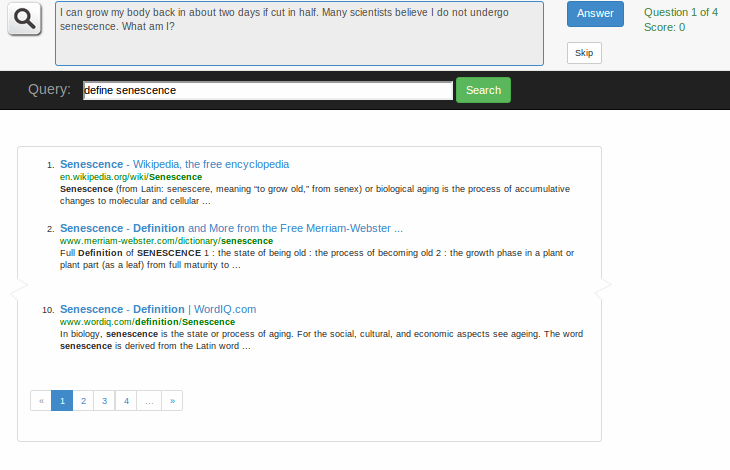
\includegraphics[scale=0.28]{img/ufindit}
\caption{The interface of the search game used in the study}
\label{figure:ufindit}
\end{figure}

\begin{table*}[tbh]
\centering
\caption{Search tasks used for the study, and specific search hints shown to one of the user groups}
\label{table:tasks}
\begin{tabular}{|p{1cm}|p{4.5cm}|p{4.2cm}|p{6.0cm}|} \hline
 & Question & Correct Answer & Specific hints \\ \hline
Task 1 & I can grow body back in about two days if cut in half. Many scientists think I don't undergo senescence. What am I? & Senescence means ``biological aging''. Hydra is considered biologically immortal and regenerates fast. & \parbox[t]{6cm}{
1. Find what is senescence\\
2. Find who does not undergo senescence\\
3. Find who can also regenerate body and choose the one that satisfies both conditions} \\ \hline
Task 2 & Of the Romans "group of three" gods in the Archaic Triad, which one did not have a Greek counterpart? & Archaic Triad includes Jupiter, Mars and Quirinus. Among those Quirinus didn't have a Greek counterpart. &
\parbox[t]{6cm}{
1. Find the names of the gods from the Archaic triad\\
2. For each of the gods find a Greek counterpart
}\\ \hline
Task 3 & As George surveyed the ``waterless place'', he unearthed some very important eggs of what animal? & "Gobi" in Mongolian means ``Waterless place''. The first whole dinosaur eggs were discovered there in 1923. & \parbox[t]{6cm}{
1. Find what is the ``waterless place'' mentioned in the question?\\
2. Search for important eggs discovery in this ``waterless place''}\\ \hline
Task 4 & If you were in the basin of the Somme River at summers end in 1918, what language would you have had to speak to understand coded British communications? & Cherokee served as code talkers in the Second Battle of the Somme. & \parbox[t]{6cm}{
1. Find the name of the battle mentioned in the questions\\
2. Search for which coded communications language was used in this battle\\
} \\ \hline
\end{tabular}
\end{table*}

Search engines are ubiquitous, and millions of people of varying experience use them on daily basis.
Unfortunately, not all searches are successful. Bilal and Kirby \cite{Bilal:2002:DSI:637512.637516} reported that about half of the participants of their user study felt frustration when searching.
Xie and Cool \cite{xie2009understanding} demonstrated that most of the time users have problems with formulating and refining search queries.
Besides good retrieval performance, a successful search requires users to possess certain skills.
Search skills can be trained, e.g. Google offers a course\footnote{http://www.powersearchingwithgoogle.com} on improving search efficiency.
Although very useful, such courses are time consuming and detached from real search problems of these particular users.
Displaying search hints is another technique that has both learning effect, and offers immediate assistance to the user in solving her current search task.
Moraveji et al. \cite{Moraveji:2011:MIU:2009916.2009966} demonstrated that hints, suggesting certain search engine functionality, help people find answers more quickly, and the effect is retained after a week without hints.

% Besides the awareness about search tools available, adopting general search strategies is extremely important when dealing with a difficult search task.
In this paper we focus on {\em strategic} search hints, that are designed to guide a user in solving her search problem.
More specifically, we chose the divide-and-conquer strategy, i.e., splitting an original difficult question into smaller problems, searching answers to the subtasks and combining them together.
Two sets of strategic hints were manually designed: {\em generic} hints describing the divide-and-conquer strategy in general and {\em task-specific} hints providing a concrete strategy to solve the current search task.
To evaluate the effect of the hints on behavior and search success we conducted a user study with 90 participants.
The results of the user study, described in this paper, demonstrate that well-designed task-specific hints can improve search success rate.
In contrast, generic search hints, which were too general and harder to follow, had negative effect on user performance and satisfaction.
% Our performance-based results were complemented with post-study surveys, which indicated that while search hints could make the search easier and more successful, they do not necessarily make it more enjoyable, suggesting that further exploration is needed into both what kind of assistance a search engine could provide, and when it would be most welcome.

\section{Related Work}

There has been considerable amount of work on search assistance and improving user experience with feedback, suggestions and hints.
Results of the study in \cite{xie2009understanding} demonstrate that in 59.5\% of the cases users need help to refine their searches or to construct search statements.
% That confirms findings of \cite{Holscher2000337}.
Individual term (\cite{ruthven2003survey}) or query suggestion (\cite{Bhatia:2011:QSA:2009916.2010023, Cao:2008:CQS:1401890.1401995,Jones:2006:GQS:1135777.1135835}) are among the most popular techniques for helping users to augment their queries.
The study in \cite{Kelly:2009:CQT:1571941.1572006} demonstrated that users prefer query suggestions over term relevance feedback, and that good manually designed suggestions improve retrieval performance.
Query suggestion methods usually use search logs to extract queries that are similar to the query of interest and work better for popular information needs \cite{Bhatia:2011:QSA:2009916.2010023}.

When query or term suggestions are not efficient, it is still possible to help users by providing potentially useful search hints.
An adaptive tool providing tactical suggestions was presented in \cite{Kriewel2010} and users reported overall satisfaction with its automatic non-intrusive advices.
Modern search engines have many features that are not typically used by an average user, but can be very useful in particular situations as shown in \cite{Moraveji:2011:MIU:2009916.2009966}. The study demonstrated the potential effectiveness and teaching effect of hints.
The major difference of our work from \cite{Moraveji:2011:MIU:2009916.2009966} is the type of search hints used.
Rather than suggesting to users the available search functionality, this work focuses on {\em strategic} search hints, designed to solve difficult informational questions.

\section{User Study}

To estimate the effect of strategic search hints on user behavior we conducted a study in a form of a web search game similar to ``a Google a Day''\footnote{http://www.agoogleaday.com/} and uFindIt \cite{Ageev:2011:FYG:2009916.2009965}. Participants were hired using Amazon Mechanical Turk\footnote{http://www.mturk.com/}. 

% \subsection{Web Search Game}
The goal of the web search game used in the user study is to find answers to several questions with the provided web search interface (Figure \ref{figure:ufindit}). 
Players are instructed not to use any external tools.
% Figure \ref{figure:ufindit} shows the interface of the game.
The questions are given one by one and since tasks might be too difficult, a chance to skip a question was provided, although users were instructed that effort put into solving a question will be evaluated.
To answer a question each player needs to provide a link to a page containing the answer as well as its text.
The answer is automatically verified and a popup box notifies a player if the answer is incorrect (since the answer can be formulated differently, presence of a keyword was checked).
A player can then continue searching or skip the question when she gives up.
A bonus payment was made to players who answer all questions correctly.
We used Bing Search API\footnote{http://www.bing.com/toolbox/bingsearchapi} as a back-end of the game search interface.
All search results and clicked documents were cached so users asking the same query or clicking the same page got the same results.
At the end of the game a questionnaire was presented asking for feedback on user satisfaction with the game, prior experience and other comments.

% \subsection{Search Tasks Description}
The tasks for the study were borrowed from the ``A Google a Day'' questions archive.
Such questions are factual, not ambiguous and usually hard to find the answer with a single query, which makes them interesting for user assistance research.
% Unfortunately, a lot of web pages discussing solutions to these questions exist.
We filtered search results to exclude all pages that discuss solutions to ``A Google a Day'' puzzles.
To do this we removed pages that mention a major part of the search question or ``a google a day'' phrase.
To keep users focused throughout the whole game we limited the number of questions to 4.
The tasks are described in Table \ref{table:tasks} and were presented to all participants in the same order to ensure comparable learning effects.

%\subsection{Search Tips}
% The questions used for the game are examples of difficult informational search tasks, which are hard to answer with a single search.
The questions have multiple parts and to solve them it is helpful to search for answers to parts of the questions and then combine them.
In one of the previous studies we observed, that most of the users didn't adopt the divide-and-conquer strategy, but kept trying to find the ``right'' query.
We decided to estimate the effect of strategic search hints, suggesting users to adopt the new strategy.

We built 2 sets of strategic hints: {\em task specific} and {\em generic}.
Task-specific hints described steps of one of the possible solutions to each question (Table \ref{table:tasks}).
Second set contained a single hint, which was shown for all tasks. Generic hint described the divide-and-conquer strategy:\\
% \begin{tabular}{|p{8cm}|}
\vspace{-2mm}
\hrule
\vspace{-2mm}
\begin{enumerate} \itemsep0pt \parskip0pt \parsep0pt
\item Split the question into 2 or more logical parts
\item Find answers to the parts of the question
\item Use answers to the parts of the question to find answer to the full question
\end{enumerate}
\vspace{-2mm}
For example, the question: ``The second wife of King Henry VIII is said to haunt the grounds where she was executed. What does she supposedly have tucked under her arm?''
\begin{enumerate} \itemsep0pt \parskip0pt \parsep0pt
\item Search [second wife King Henry VIII] to find Anne Boleyn.
\item Search [Anne Boleyn under arm] to find that her ghost is in the London Tower where she is said to carry her head tucked underneath her arm.
\end{enumerate}
\vspace{-1mm}
\hrule
% \end{tabular}
\vspace{+2mm}
To control for the learning effect demonstrated in \cite{Moraveji:2011:MIU:2009916.2009966}, each user was assigned to one of the three groups:
\vspace{-2mm}
\begin{enumerate}
\item users who didn't get any hints
\vspace{-2mm}
\item users who got task-specific hints
\vspace{-2mm}
\item users who got the generic hints
\end{enumerate}
% During the game tips were displayed in the right panel of the search interface (Figure \ref{figure:ufindit}).

\section{Results}

% First we describe the general task completion statistics for participants overall, then dive into performance for different cohorts, comparing task success, time to completion, number of attempted answers.
% We complement this performance-based analysis with subjective survey-based impressions of the searchers.

From 199 unique participants, who clicked the HIT on Amazon Mechanical Turk only 90 players finished the game.
We further examined all games manually and filtered out 9 submissions for one of the following reasons: lack of effort (e.g. skipped several tasks after none or a single query) or usage of external resources (e.g. the answer was obtained without submitting any queries or results explored didn't contain the answer).
Furthermore, 10 players from the group which received hints indicated in the survey that they didn't see them, so we filtered out those submissions and finally we had 71 completed games (29 for no hints, 20 for task-specific hints and 22 for generic hints groups).

\vspace{-1mm}
\subsection{Effects of Search Tips on Performance}

In order to measure search success rate we looked at the number of questions answered correctly by different groups of users\footnote{Since users were allowed to skip a question we are counting the number of questions that were eventually solved correctly even if a player made some incorrect attempts}.
Figure \ref{figure:task_success} shows that success rate is higher for users who saw task-specific hints compared to users who didn't get such assistance.
Surprisingly, having the generic hint decreased the success rate, although users could easily ignore a hint they didn't like.
A possible explanation is: generic hints were harder to follow and users who tried and failed became frustrated and didn't restart their searches.

% Similar to \cite{Moraveji:2011:MIU:2009916.2009966} we looked at the average time to answer a question (for this analysis we removed games where a user didn't find the answer and skipped the task).

The plot of average time to answer a question on Figure \ref{figure:task_time} doesn't show an improvement for the task-specific hints group, except for the question 1.
Our task-specific hints represent a possible way to solve a problem and there is no guarantee, that it is the fastest one.
It is worth noting, that users from the generic search hint group had slightly higher variance in success time, which can probably be explained by the fact that some users were successful in finding the right way to follow the hint and some other users struggled with it much longer.
Another insight comes from the number of incorrect attempts users made.
Figure \ref{figure:incorrect} demonstrates the average number of incorrect answer attempts for all groups of users.
Although the variance is high, there is a tendency for users who saw task-specific hints to make less attempts than both other groups.
This is not in direct correspondence with time spent on the game.
It seems that the users who saw a clear strategy to solve the question were less likely to notice plausible, but incorrect solution.
Moreover, we analyzed texts of incorrect answers, and can conclude that a big part of incorrect submission are due to users trying all possible options they found on the way, even if these options are clearly wrong.
% We should note, that unfortunately we didn't limit the number of attempts per problem, thus strategy to verify an answer by submitting it made sense.

\begin{figure}[H]
\centering
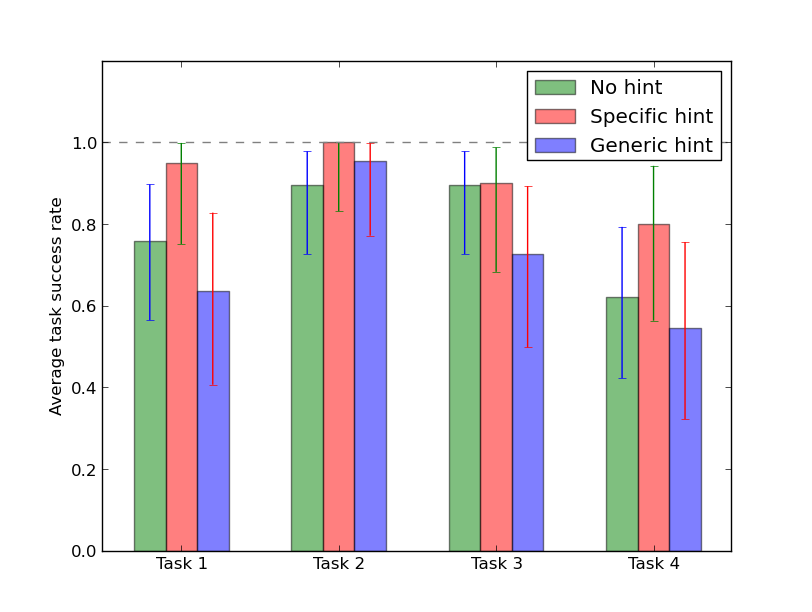
\includegraphics[scale=0.33]{img/success_per_task}
\caption{Success rate per task for each group of participants}
\label{figure:task_success}
\end{figure}
\vspace{-6mm}
\begin{figure}[H]
\centering
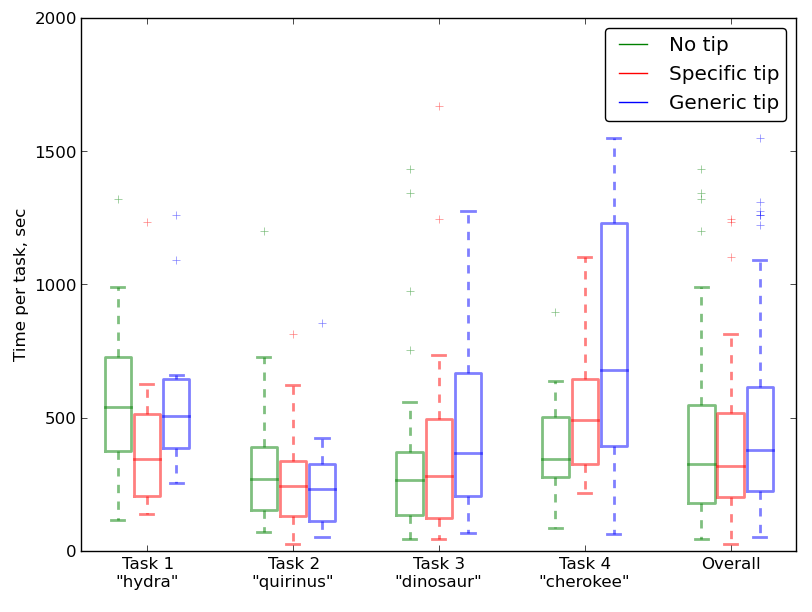
\includegraphics[scale=0.35]{img/time_per_task}
\caption{Task completion time for each group of players}
\label{figure:task_time}
\end{figure}
\vspace{-6mm}
\begin{figure}[H]
\centering
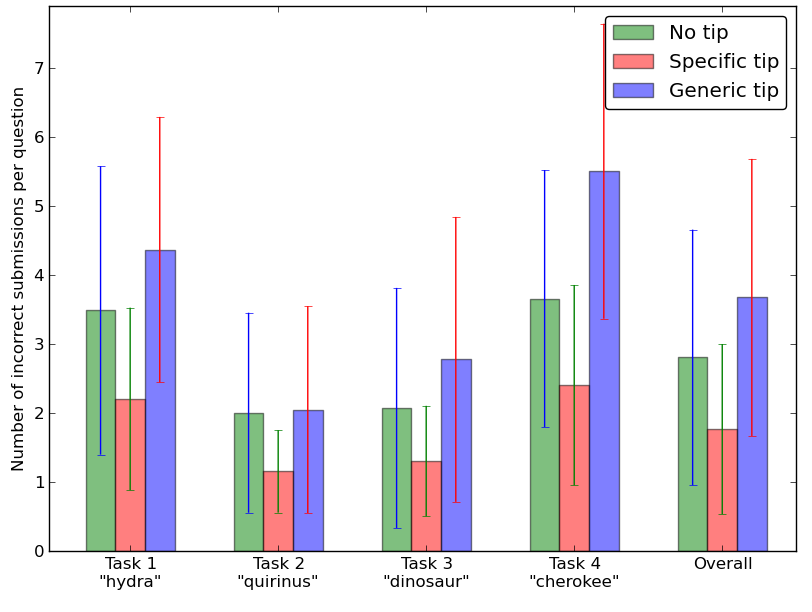
\includegraphics[scale=0.33]{img/incorrect}
\caption{The number of incorrect submission attempts per question for all groups of users}
\label{figure:incorrect}
\end{figure}
\begin{figure*}[ht]
\centering
\begin{subfigure}[t]{0.3\textwidth}
	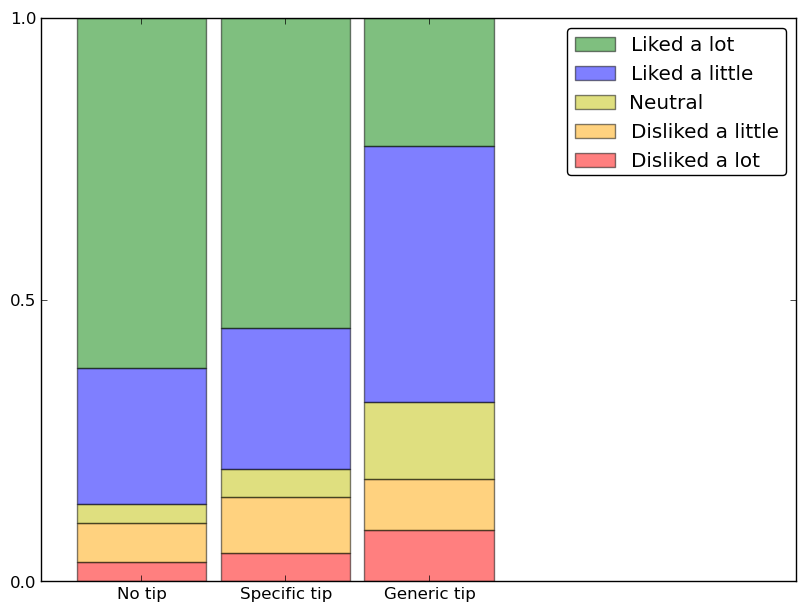
\includegraphics[scale=0.26]{img/liked}
	\caption{How did you like the game?}
    \label{figure:survey:liked}
\end{subfigure}
\begin{subfigure}[t]{0.3\textwidth}
	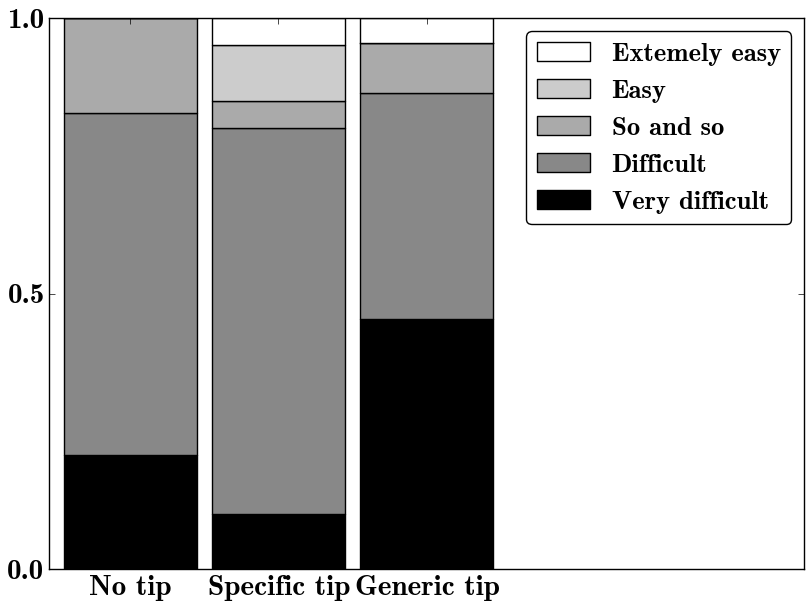
\includegraphics[scale=0.26]{img/difficult}
	\caption{How difficult was the game?}
    \label{figure:survey:difficult}
\end{subfigure}
\begin{subfigure}[t]{0.3\textwidth}
	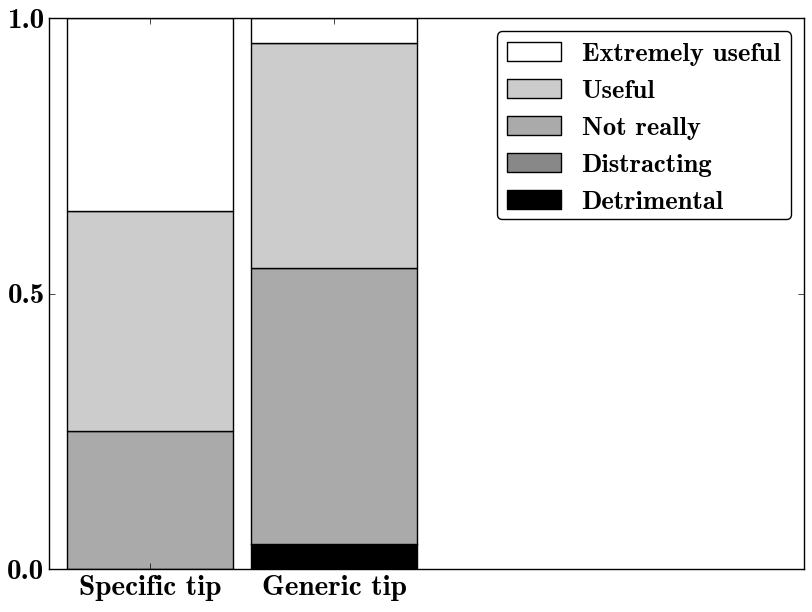
\includegraphics[scale=0.26]{img/useful}
	\caption{Were search hints useful to you?}
    \label{figure:survey:useful}
\end{subfigure}
\vspace{-2mm}
\caption{Proportions of replies to some of the survey question for each group of users}
\label{figure:survey}
\vspace{-4mm}
\end{figure*}

\vspace{-3mm}
We also looked at other search behavior characteristics: number of queries submitted, number of clicks made, average length of the queries. The variance in these characteristics was too high to make any speculations regarding their meaning.

\subsection{Effects of Search Tips on User Experience}

Finally, we looked at the surveys filled out by each group of users.
Figure \ref{figure:survey} presents proportions of different answers to three of the questions: ``How did you like the game?'', ``How difficult was the game?'' and ``Were search hints useful to you?''.
Surprisingly, user satisfaction with the game was lower for users who saw hints during the game and users who didn't get any assistance enjoyed it more.
The replies to the question about game difficulty are in agreement with the success rate: users who saw task-specific hints rated difficulty lower than participants who struggled to find the correct answers.
The game was very difficult on average, however, some participants from the group who received task-specific hints surprisingly rated it as very easy, which suggests that our hints do help users.
This is supported by the answers to the last question on whether hints were helpful (Figure \ref{figure:survey:useful}).

To summarize, the results of the conducted user study suggest that specific search hints can be helpful, which is indicated by higher success rate, lower number of incorrect attempts and positive feedback in the end of study survey.
In contrast, generic hints can have negative effect on user experience, which is indicated by lower success rate, increased number of incorrect attempts and higher perceived tasks complexity according to the survey.

\vspace{-1mm}
\section{Conclusion}
In this paper we studied the effect of strategic search hints on user behavior. 
The conducted user study in a form of a web search game demonstrated the potential of good hints in improving search success rate.
However, to be useful, they should be designed carefully.
Search hints that are too general can be detrimental to search success.
We also find that even searchers who are more effective using specific search hints, feel subjectively less satisfied and engaged than the control group, indicating that search assistance has to be specific and timely if it is to improve the searcher experience.
% The results of the study have important implications for designing an effective search engine assistance/dialogue.

We should note, that specific search hints used in this work were manually generated and an interesting question of future work is how to generate such useful hints automatically.
It should be possible to learn strategies applied by the experienced search users and suggest them to the rest.

% Our performance-based results were complemented with post-study surveys, which indicated that while search hints could make the search easier and more successful, they do not necessarily make it more enjoyable, suggesting that further exploration is needed into both what kind of assistance a search engine could provide, and when it would be most welcome.

% ACKNOWLEDGMENTS are optional
\vspace{-1mm}
\section{Acknowledgments}
The authors would like to thank Daniel Russel for providing an archive of questions from ``a Google a Day'' search game. This work was supported by the DARPA CSSG prorgram through grants N11AP20012 and D11AP00269.

%
% The following two commands are all you need in the
% initial runs of your .tex file to
% produce the bibliography for the citations in your paper.
\bibliographystyle{abbrv}
\bibliography{sigproc}  % sigproc.bib is the name of the Bibliography in this case
% You must have a proper ".bib" file
%  and remember to run:
% latex bibtex latex latex
% to resolve all references
%
% ACM needs 'a single self-contained file'!
%
%APPENDICES are optional
%\balancecolumns

\end{document}
